% En esta seccion se presentan experimentos concretos efectuados, exitosos o fallidos, mediante figuras y capturas de pantalla debidamente tituladas y referenciadas en el cuerpo del reporte.
\section{Experimentos}

\subsection{Actividad 1: Plano paralelo al plano XY}
La primera prueba se hizo descomentando el bloque del plano tal como viene en el
proyecto base, es decir, con \texttt{Plane plane(1.0f)}. El plano apareció en
pantalla y quedó centrado en el origen, pero era visiblemente más chico de lo
que pedía el manual: sus vértices caen en $\pm0.5$, de modo que el lado mide una
unidad y no dos. En la Figura \ref{fig:actividad1-tamano} se comparan las dos
llamadas con la cámara en la misma posición, y se aprecia que el plano correcto
ocupa exactamente el doble de lado que el del proyecto base. La confusión viene
de que el parámetro parece ser el semilado, cuando en realidad el constructor
lo divide entre dos internamente; sólo al ver que las aristas del plano no
coincidían con las marcas de los ejes coordenados nos dimos cuenta del error.

\begin{figure}[H]
    \centering
    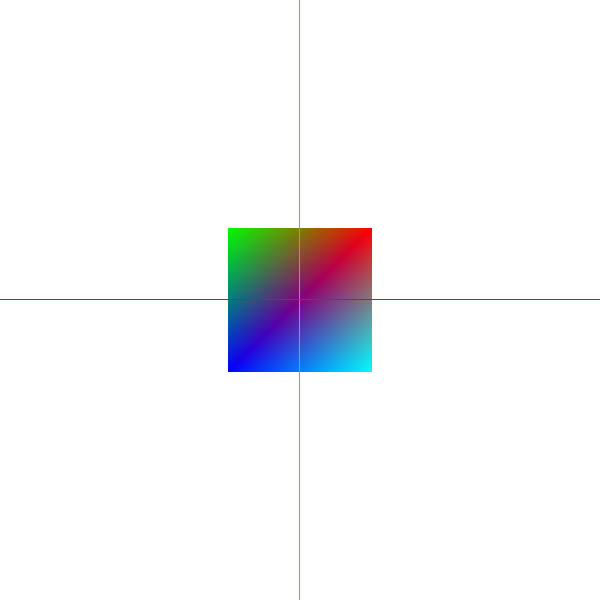
\includegraphics[width=0.45\textwidth]{Imagenes/E1/Plano_Base1x1.png}
    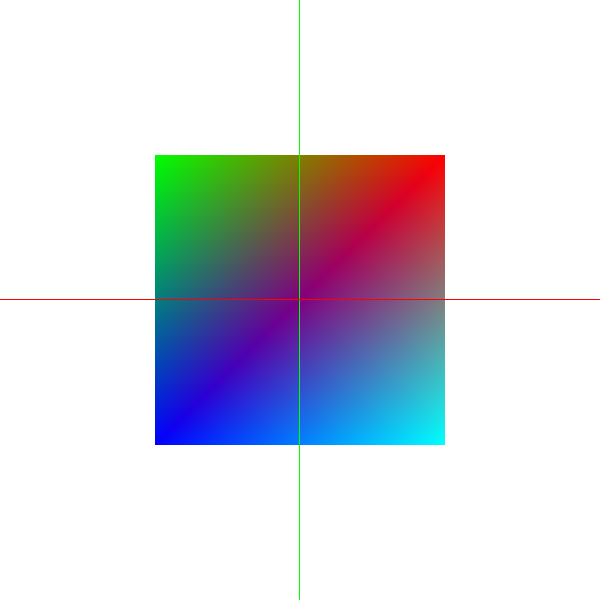
\includegraphics[width=0.45\textwidth]{Imagenes/E1/Plano_Frontal.png}
    \caption{Comparación del tamaño del plano con la cámara fija en la vista frontal: a la izquierda, \texttt{Plane(1.0f)}, el valor que trae comentado el proyecto base, que produce un plano de $1\times1$; a la derecha, \texttt{Plane(2.0f)}, que produce el plano de $2\times2$ unidades que pide el manual.}
    \label{fig:actividad1-tamano}
\end{figure}

Con el tamaño ya correcto probamos las dos vistas. Con \texttt{F1} el plano se ve
como un cuadrado perfecto, porque la cámara está sobre el eje $+Z$ y el plano es
paralelo al plano $XY$; con \texttt{F2} la misma figura se ve como un
paralelogramo, y es ahí donde se confirma que lo que hay en la escena es un
objeto plano y no un cuadrado dibujado sobre la ventana. Ambas vistas aparecen
en la Figura \ref{fig:actividad1-vistas}.

Un detalle inesperado apareció en la vista frontal: las líneas de los ejes $X$ y
$Y$ se siguen viendo \emph{encima} del plano, con su color íntegro, en lugar de
quedar tapadas por él. Al principio pensamos que era una transparencia mal
configurada. La explicación resultó más simple: los ejes y el plano están los dos
contenidos en $z=0$, es decir, exactamente a la misma profundidad, y como los
ejes se dibujan primero y la prueba de profundidad usa \texttt{GL\_LESS}, los
fragmentos del plano no pasan la prueba en esos píxeles. Lo comprobamos midiendo
el color de los píxeles sobre la línea, que resultó ser rojo puro
$(255,0,0)$ y verde puro $(0,255,0)$, sin mezclarse con el degradado del plano.

\begin{figure}[H]
    \centering
    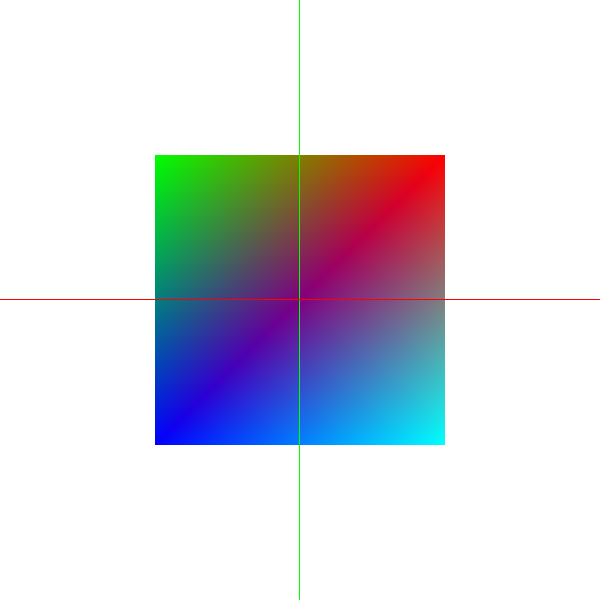
\includegraphics[width=0.45\textwidth]{Imagenes/E1/Plano_Frontal.png}
    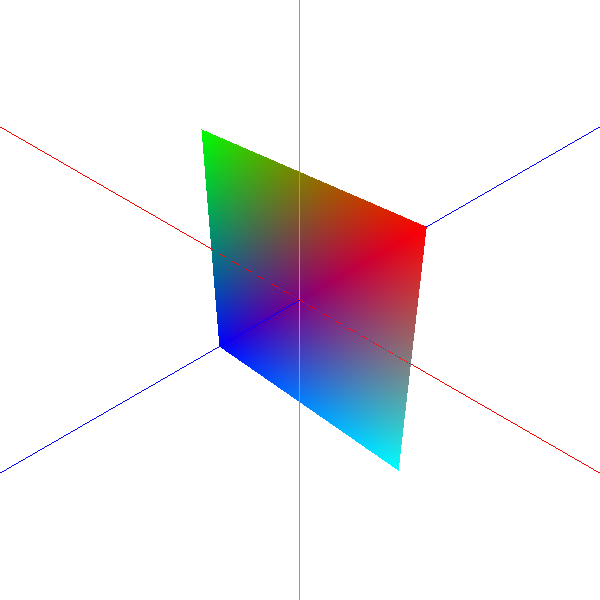
\includegraphics[width=0.45\textwidth]{Imagenes/E1/Plano_Oblicua.png}
    \caption{Las dos perspectivas del plano de $2\times2$: vista frontal con \texttt{F1} (izquierda) y vista oblicua con \texttt{F2} (derecha).}
    \label{fig:actividad1-vistas}
\end{figure}

Por último activamos el modo de alambre con la tecla \texttt{L} para verificar la
descomposición. La Figura \ref{fig:actividad1-alambre} muestra las dos aristas
del contorno y la diagonal que separa los dos triángulos, que es exactamente lo
que declara el arreglo de índices.

\begin{figure}[H]
    \centering
    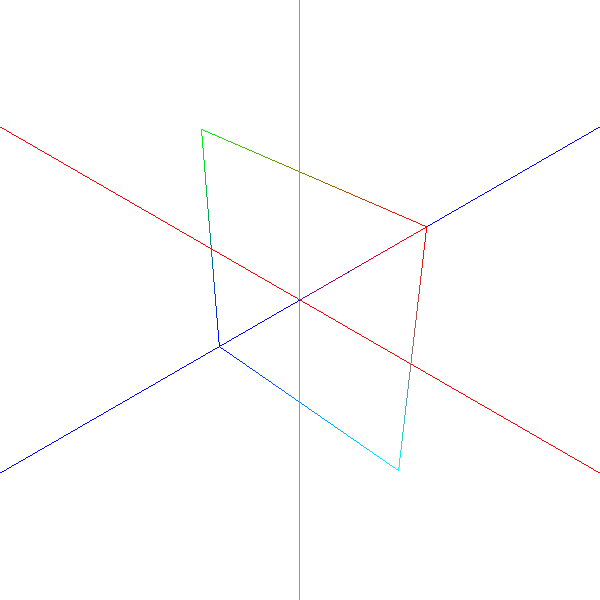
\includegraphics[width=0.45\textwidth]{Imagenes/E1/Plano_Alambre.png}
    \caption{El plano en modo de alambre: se distinguen los cuatro vértices del contorno y la diagonal que divide la figura en dos triángulos.}
    \label{fig:actividad1-alambre}
\end{figure}

\subsection{Actividad 2: Cubo centrado en el origen}
El cubo repitió la misma historia del tamaño: con \texttt{Cube(1.0f)}, el valor
del proyecto base, la arista mide una unidad en lugar de dos. Como ya
sabíamos qué buscar, esta vez la corrección fue inmediata; la comparación se
muestra en la Figura \ref{fig:actividad2-tamano}. Aprovechamos además la vista
oblicua para comprobar que la figura sí está centrada: los tres ejes coordenados
entran por tres aristas distintas y salen por las opuestas, lo que sólo ocurre si
el origen coincide con el centro geométrico del cubo.

\begin{figure}[H]
    \centering
    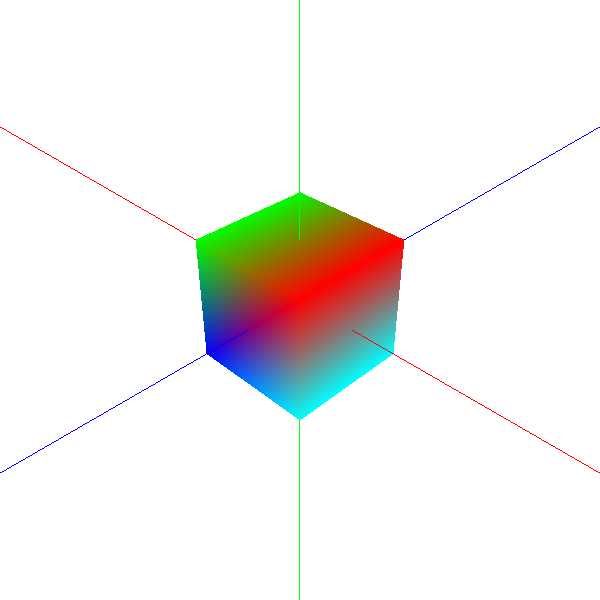
\includegraphics[width=0.45\textwidth]{Imagenes/E2/Cubo_Base1x1.png}
    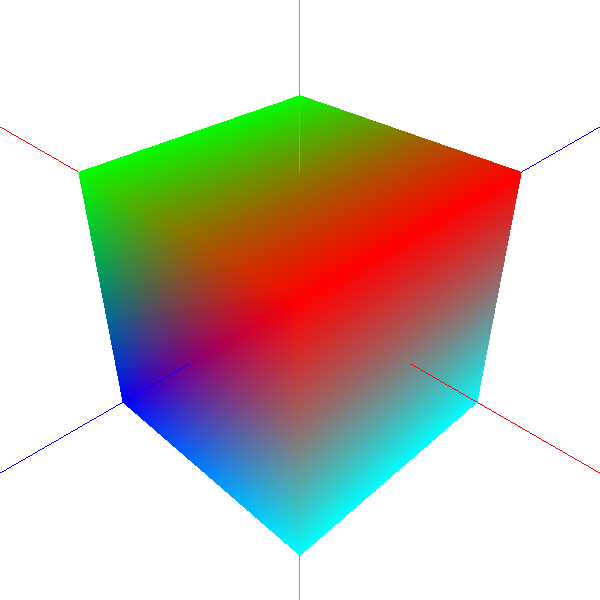
\includegraphics[width=0.45\textwidth]{Imagenes/E2/Cubo_Oblicua.png}
    \caption{Efecto del argumento del constructor sobre el cubo, con la cámara fija en la vista oblicua: \texttt{Cube(1.0f)} a la izquierda y \texttt{Cube(2.0f)} a la derecha.}
    \label{fig:actividad2-tamano}
\end{figure}

La prueba que más nos interesaba era la de las caras. En la vista frontal
(Figura \ref{fig:actividad2-vistas}, izquierda) el cubo se ve como un cuadrado y
resulta imposible saber si tiene seis caras o sólo una: la silueta sería idéntica
en ambos casos. Al pasar a la vista oblicua aparecen tres caras al mismo tiempo y
la figura se reconoce como un volumen, pero incluso así hay tres caras que no se
ven nunca. Por eso recurrimos al modo de alambre, que se muestra en la Figura
\ref{fig:actividad2-alambre}: como en ese modo no hay superficies rellenas que
oculten nada, se ven simultáneamente las aristas del frente y las del fondo, y aparece
una diagonal por cada una de las seis caras, que es lo que confirma que todas
están formadas por dos triángulos y que ninguna quedó sin cubrir.

\begin{figure}[H]
    \centering
    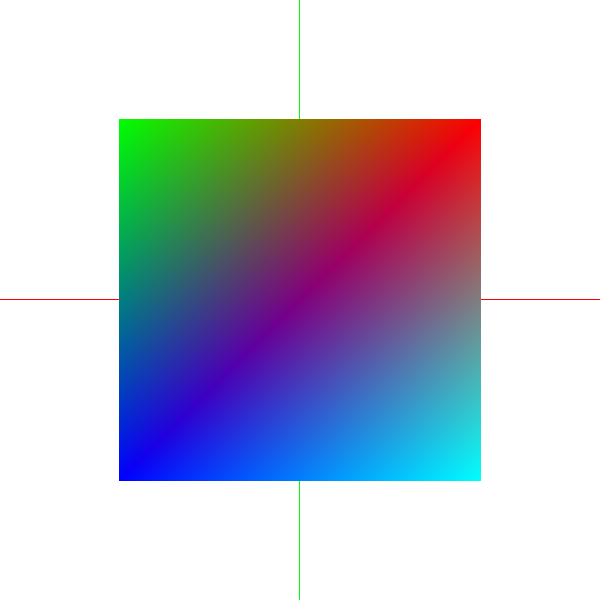
\includegraphics[width=0.45\textwidth]{Imagenes/E2/Cubo_Frontal.png}
    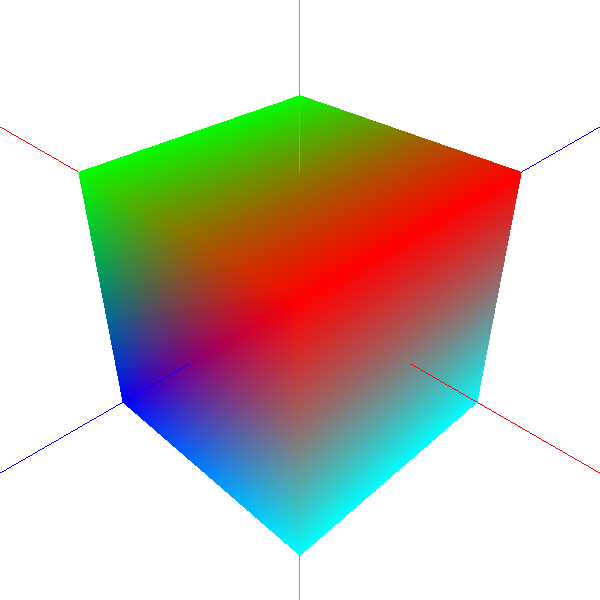
\includegraphics[width=0.45\textwidth]{Imagenes/E2/Cubo_Oblicua.png}
    \caption{Las dos perspectivas del cubo de $2\times2\times2$: vista frontal con \texttt{F1} (izquierda), en la que la figura es indistinguible de un cuadrado, y vista oblicua con \texttt{F2} (derecha), en la que se aprecian tres caras.}
    \label{fig:actividad2-vistas}
\end{figure}

\begin{figure}[H]
    \centering
    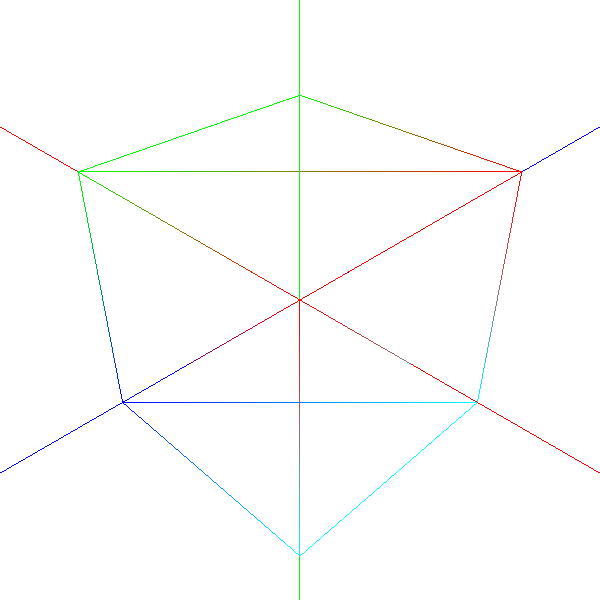
\includegraphics[width=0.45\textwidth]{Imagenes/E2/Cubo_Alambre.png}
    \caption{El cubo en modo de alambre desde la vista oblicua. Al no haber caras rellenas, se ven también las aristas del fondo y las diagonales de cada cara.}
    \label{fig:actividad2-alambre}
\end{figure}

\subsection{Actividad 3: Círculo de radio unitario}
Esta actividad fue la que dio más material. Empezamos ejecutando la clase
\texttt{Circle} tal como viene en el proyecto base y el resultado, que se muestra
en la Figura \ref{fig:actividad3-base}, no fue el que esperábamos: en lugar del
degradado continuo que produce la interpolación de colores entre vértices, el
círculo apareció dividido en tres sectores de color plano, con transiciones
abruptas justo en los $0^\circ$, $120^\circ$ y $240^\circ$.

Al leer la clase encontramos la causa. El lazo asigna color únicamente a los
vértices de esos tres ángulos y deja los demás sin escribir, y como
\texttt{Vertex} es una estructura sin constructor, declararla dentro del lazo no
inicializa sus miembros \cite{cppreference_init}. En nuestra compilación la
variable ocupa siempre la misma posición de la pila, de modo que cada vértice
hereda el color del anterior y el resultado son los tres sectores planos que se
observan; es importante subrayar que se trata de un valor indeterminado y que con
otro compilador, u otra configuración, la imagen podría ser distinta.
Ése fue el experimento que más nos costó interpretar, porque durante un rato
buscamos el problema en el shader y no en la construcción de los vértices.

\begin{figure}[H]
    \centering
    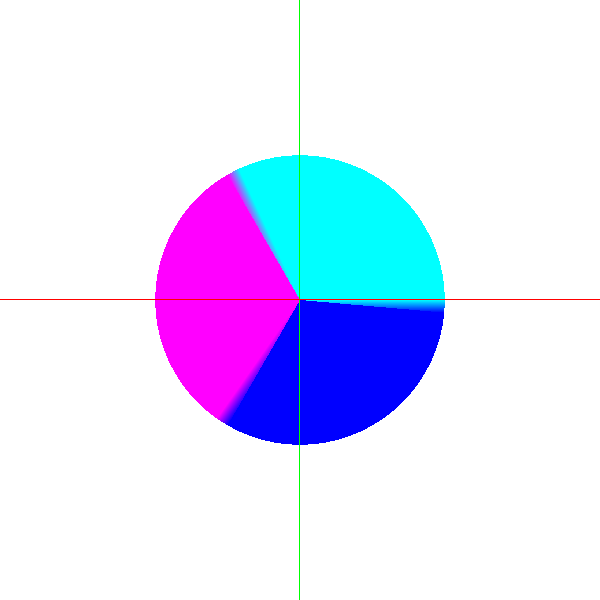
\includegraphics[width=0.45\textwidth]{Imagenes/E3/Circulo_Base.png}
    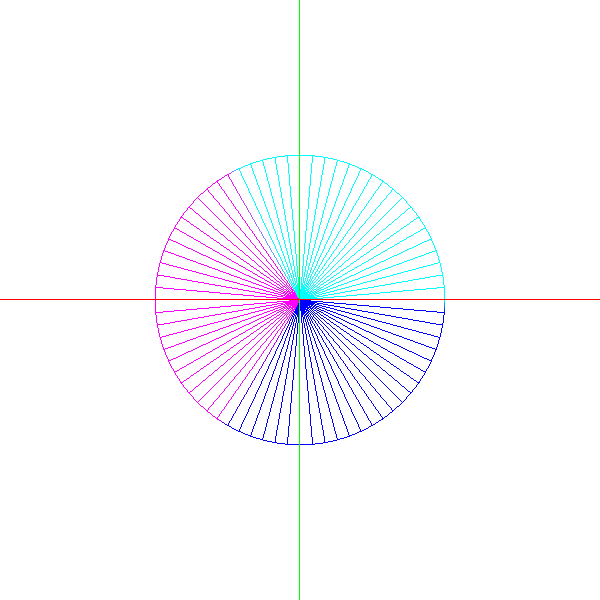
\includegraphics[width=0.45\textwidth]{Imagenes/E3/Circulo_Base_Alambre.png}
    \caption{Resultado de la clase \texttt{Circle} del proyecto base: a la izquierda, los tres sectores de color plano que produce dejar sin inicializar el color de la mayoría de los vértices; a la derecha, la misma figura en modo de alambre, donde se aprecia que todos los triángulos del abanico convergen en el centro.}
    \label{fig:actividad3-base}
\end{figure}

El segundo hallazgo no era visible en pantalla y apareció al contar los arreglos
que genera la clase. Se instrumentó el programa para imprimir su tamaño y el
índice más grande que emplea, con el resultado siguiente:

\begin{lstlisting}[language=C, caption={Salida de la instrumentacion de las dos versiones de la clase Circle}, label=lst:salida-circulo]
Circle base : 144 vertices, 435 indices, indice maximo = 144
Circle nueva: 73 vertices, 216 indices
\end{lstlisting}

Los dos números de la primera línea son problemáticos. Por un lado, la clase
genera 144 vértices para una figura que necesita 73, porque duplica el vértice
del centro una vez por cada punto del contorno; ese desperdicio explica también
por qué su segundo lazo de índices no dibuja nada, ya que todos los triángulos
que arma tienen dos de sus tres vértices en el centro y quedan degenerados. Por
otro lado, y esto es lo grave, el índice más grande que utiliza es el 144,
mientras que los índices válidos van del 0 al 143: la clase le pide a OpenGL un
vértice que no existe. Este error no produjo ningún síntoma visible en nuestro
equipo, lo cual lo vuelve más peligroso que el de los colores, porque nada en la
imagen delata que está ahí.

Con la clase reescrita repetimos las pruebas. La Figura
\ref{fig:actividad3-vistas} muestra las dos vistas: con \texttt{F1} se obtiene el
círculo y con \texttt{F2} la misma figura se proyecta como una elipse, que es
justamente lo que debe ocurrir con una figura plana observada desde un ángulo
oblicuo. El degradado ahora sí es continuo alrededor de todo el contorno.

\begin{figure}[H]
    \centering
    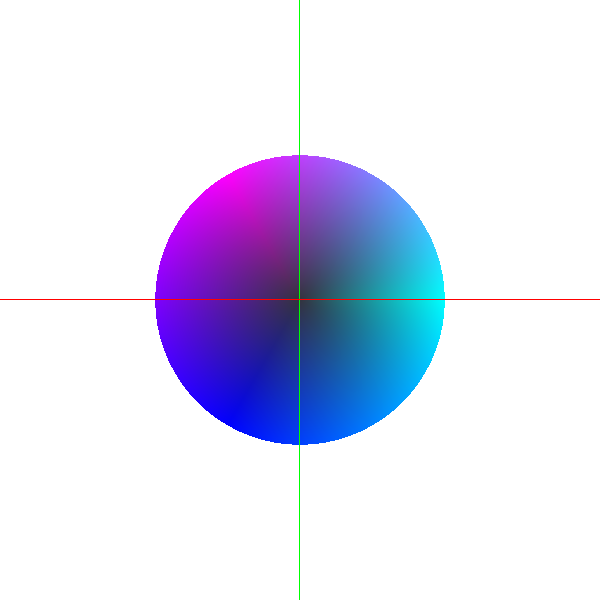
\includegraphics[width=0.45\textwidth]{Imagenes/E3/Circulo_Frontal.png}
    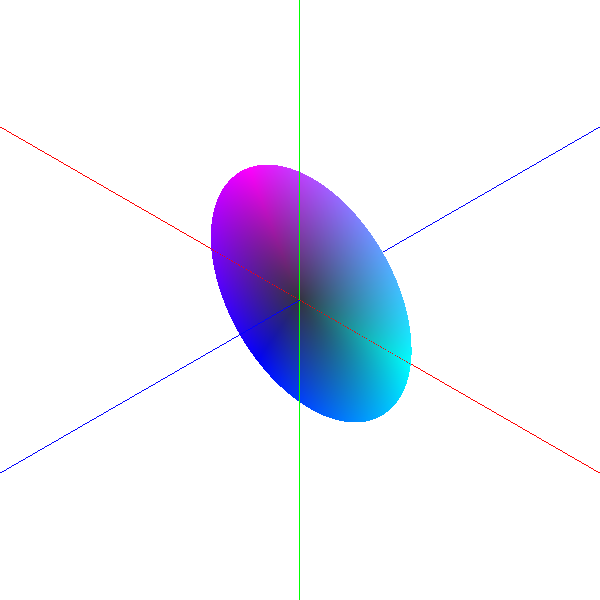
\includegraphics[width=0.45\textwidth]{Imagenes/E3/Circulo_Oblicua.png}
    \caption{Las dos perspectivas del círculo de radio unitario con la clase reescrita: vista frontal con \texttt{F1} (izquierda) y vista oblicua con \texttt{F2} (derecha), en la que la figura se proyecta como una elipse.}
    \label{fig:actividad3-vistas}
\end{figure}

El último experimento consistió en variar el número de lados del polígono con el
que se aproxima la circunferencia. Con los 72 lados que quedaron como valor
predeterminado, un vértice cada cinco grados, el contorno se ve liso a la
resolución de la ventana; al bajarlo a 12 la figura deja de parecer un círculo y
se reconoce con claridad como un polígono, tal como se aprecia en la Figura
\ref{fig:actividad3-lados}. El modo de alambre, en la Figura
\ref{fig:actividad3-alambre}, deja ver el abanico completo: 72 triángulos que
comparten el vértice del centro.

\begin{figure}[H]
    \centering
    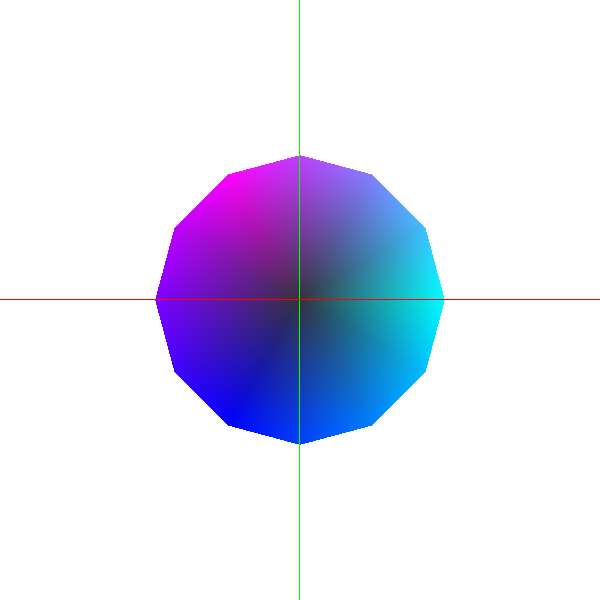
\includegraphics[width=0.45\textwidth]{Imagenes/E3/Circulo_12.png}
    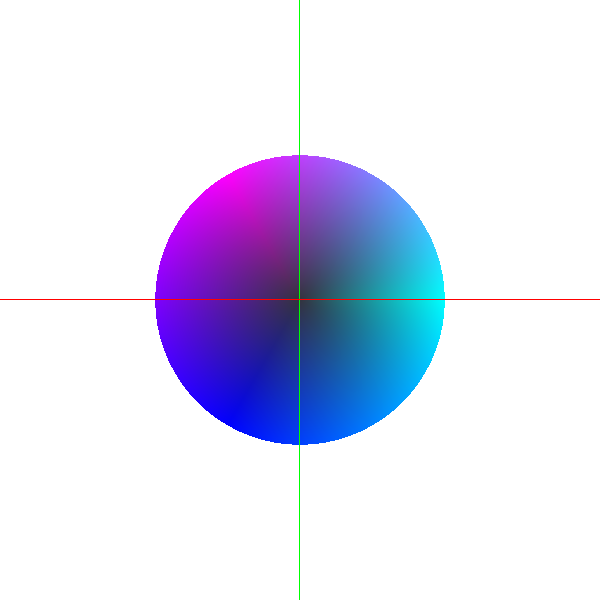
\includegraphics[width=0.45\textwidth]{Imagenes/E3/Circulo_Frontal.png}
    \caption{Efecto del número de lados sobre la aproximación de la circunferencia: con 12 lados el contorno es claramente poligonal (izquierda) y con 72 se percibe liso a la resolución de la ventana (derecha).}
    \label{fig:actividad3-lados}
\end{figure}

\begin{figure}[H]
    \centering
    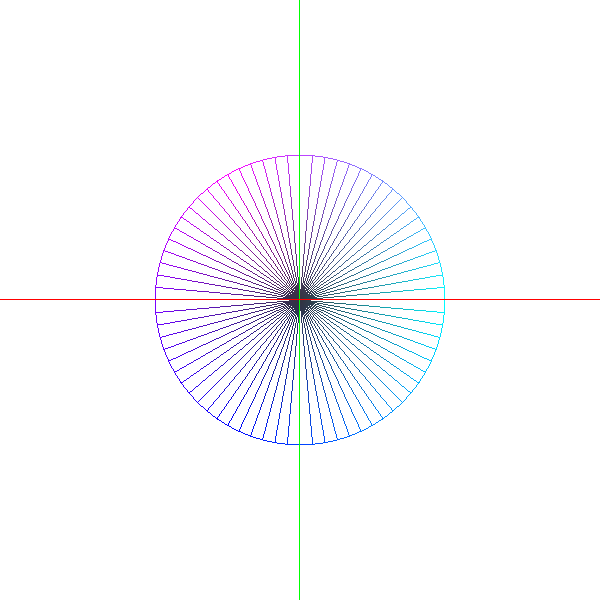
\includegraphics[width=0.45\textwidth]{Imagenes/E3/Circulo_Alambre.png}
    \caption{El círculo en modo de alambre: los 72 triángulos del abanico convergen en el único vértice del centro.}
    \label{fig:actividad3-alambre}
\end{figure}

\subsection{Actividad 4: Cilindro centrado en el origen}

Para verificar el correcto modelado del cilindro, se realizaron pruebas de ejecución modificando las condiciones de la cámara y el modo de renderizado de OpenGL. Se configuraron las teclas de función F1 y F2 para alternar entre dos puntos de vista clave.

El experimento se dividió en las siguientes fases:
\begin{enumerate}
    \item \textbf{Prueba de alineación y simetría (F1):} Se posicionó la cámara en $(0, 0, 5)$ con vista directa hacia el origen $(0, 0, 0)$. Esta perspectiva frontal permitió comprobar que el cuerpo del cilindro abarcase una unidad hacia arriba y una unidad hacia abajo sobre el eje vertical $Y$, y que sus costados coincidieran con $x = -1.0$ y $x = +1.0$.
    \item \textbf{Prueba de volumen tridimensional y sellado (F2):} Se cambió la cámara a una vista oblicua en $(4.0, 3.5, 4.5)$. Mediante esta toma se verificó que la tapa superior e inferior estuvieran construidas correctamente, y que la interpolación continua de color eliminara las caras negras del código original.
\end{enumerate}

En la Figura~\ref{fig:experimento_cilindro} se ven las tres capturas obtenidas durante las pruebas.

\begin{figure}[H]
    \centering
    \begin{minipage}{0.45\textwidth}
        \centering
        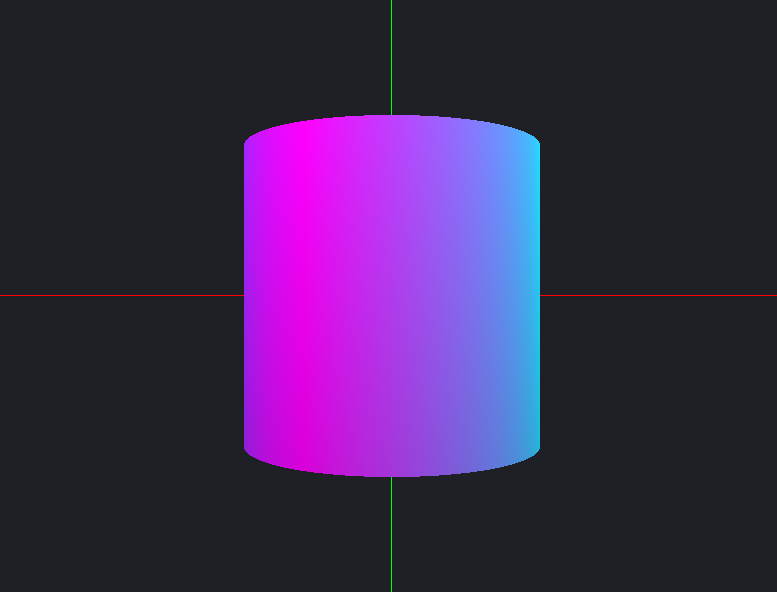
\includegraphics[width=\linewidth]{Imagenes/E4/act4_f1.png}
        \vspace{1mm}
        \centerline{\footnotesize (a) Vista frontal (F1).}
    \end{minipage}\hfill
    \begin{minipage}{0.45\textwidth}
        \centering
        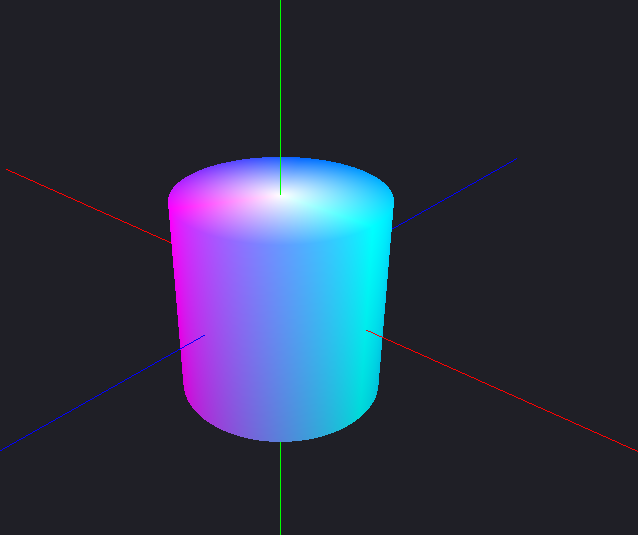
\includegraphics[width=\linewidth]{Imagenes/E4/act4_f2.png}
        \vspace{1mm}
        \centerline{\footnotesize (b) Vista oblicua (F2).}
    \end{minipage}
    \vspace{2mm}
    \caption{Pruebas experimentales del cilindro de radio 1 y altura 2 centrado en el origen.}
    \label{fig:experimento_cilindro}
\end{figure}


\subsection{Actividad 5. Esfera centrada en el origen}
Con la triangulación ya implementada, el primer experimento reveló el mismo
patrón de color que ya habíamos documentado en la Actividad 3: al dejar el
esquema de color original de la clase, sólo los tres meridianos en
$\theta = 0^\circ$, $120^\circ$ y $240^\circ$ se veían coloreados, y el resto
de la superficie aparecía en negro, con la triangulación ya correcta pero
invisible al no recibir color propio. La Figura
\ref{fig:actividad5-colorbase} lo muestra en las dos vistas.

\begin{figure}[H]
    \centering
    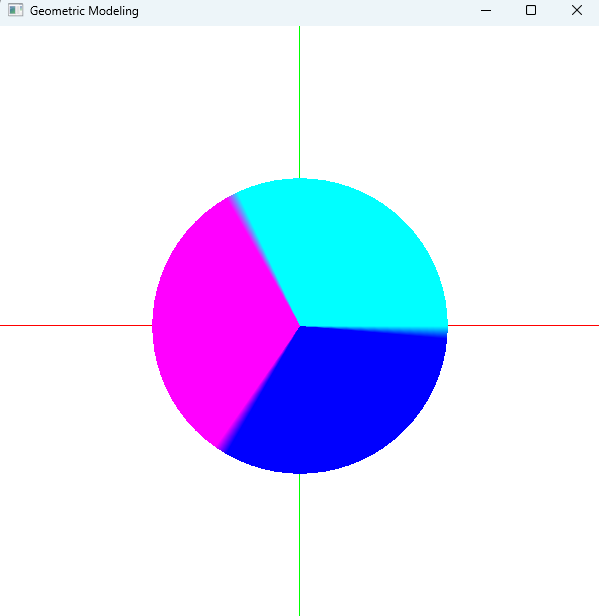
\includegraphics[width=0.45\textwidth]{Imagenes/E5/Esfera_ColorBase_Frontal.png}
    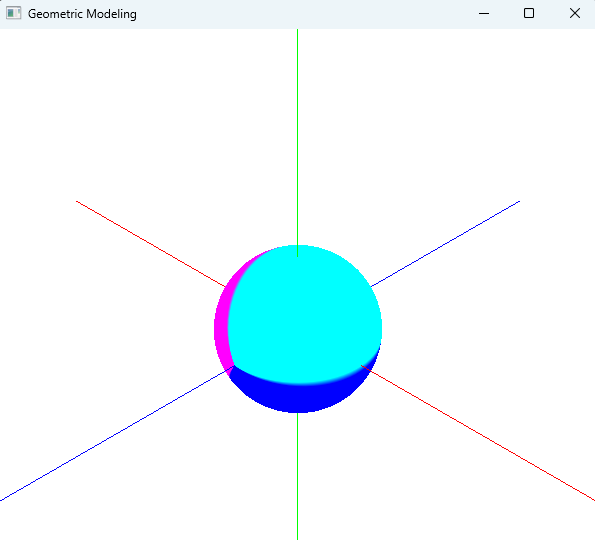
\includegraphics[width=0.45\textwidth]{Imagenes/E5/Esfera_ColorBase_Oblicua.png}
    \caption{Esfera ya triangulada pero con el esquema de color original de la clase: sólo tres meridianos reciben color y el resto de los 2592 vértices quedan sin inicializar. Vista frontal con \texttt{F1} (izquierda) y oblicua con \texttt{F2} (derecha).}
    \label{fig:actividad5-colorbase}
\end{figure}

Con el color corregido mediante el mapeo de la posición normalizada, repetimos
las pruebas de siempre. Con \texttt{F1} y \texttt{F2} se confirmó que la
esfera se ve igual de redonda desde cualquier ángulo, a diferencia del plano y
el círculo, cuya silueta sí cambiaba entre una vista y otra; esto tiene
sentido porque la silueta de una esfera es un círculo sin importar la
dirección desde la que se observe. La Figura \ref{fig:actividad5-vistas}
muestra las dos vistas con el degradado ya continuo.

\begin{figure}[H]
    \centering
    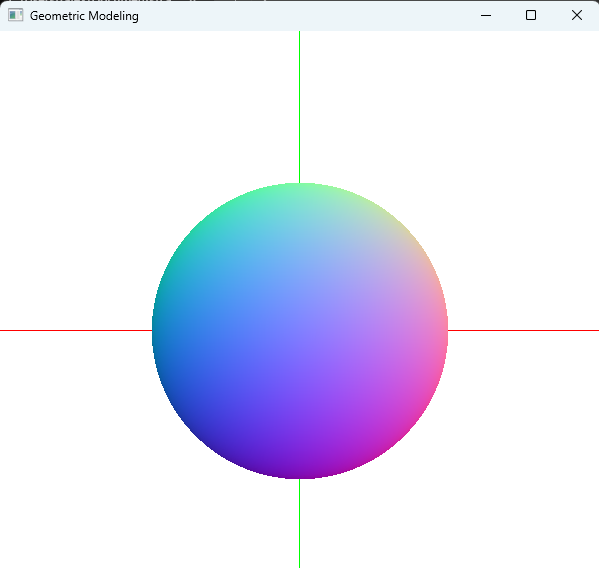
\includegraphics[width=0.45\textwidth]{Imagenes/E5/Esfera_Frontal.png}
    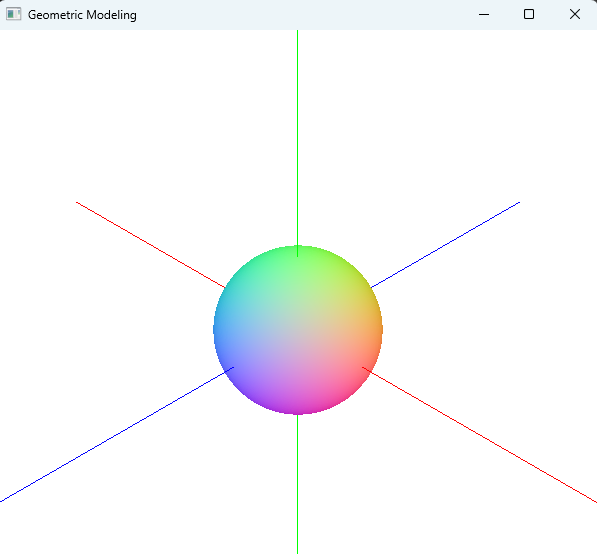
\includegraphics[width=0.45\textwidth]{Imagenes/E5/Esfera_Oblicua.png}
    \caption{Las dos perspectivas de la esfera de radio unitario, ya con el color corregido: vista frontal con \texttt{F1} (izquierda) y vista oblicua con \texttt{F2} (derecha).}
    \label{fig:actividad5-vistas}
\end{figure}

\subsection{Actividad 6: Cono centrado en el origen}

Para esta actividad, primero corrimos la clase del cono tal como venía en la plantilla que nos dieron. Nos pasó exactamente lo mismo que con el círculo: casi toda la figura se veía de color negro y sólo tenía tres líneas de color en $0^\circ$, $120^\circ$ y $240^\circ$. Al revisar el código vimos que a los demás puntos no se les había puesto color, así que la computadora no sabía de qué tono pintarlos. Además, al girar la cámara por debajo, la figura estaba completamente hueca porque le faltaba la tapa de abajo.

También revisamos los números del código y notamos que repetía la punta del cono 72 veces en el mismo lugar, gastando memoria y armando triángulos encimados que ni se veían. Por eso arreglamos la clase para ponerle un solo punto en la punta, cerrar la base redonda con su propia tapa y repartir bien los colores cian, magenta y azul.

Con la figura ya corregida, probamos las diferentes vistas del programa, las cuales se muestran en la Figura~\ref{fig:experimento_cono}:
\begin{enumerate}
    \item Con la tecla F1 pusimos la vista de frente. Como la cámara queda derecha, el cono se ve perfectamente como un triángulo plano.
    \item Con la tecla F2 pasamos a la vista de lado en diagonal. Aquí sí se nota el volumen en 3D y se comprueba que el cono está justo en medio del origen, ya que las líneas de los ejes le pasan por el centro.
    \item Con la tecla L activamos el modo de alambre. Así pudimos comprobar que todos los triángulos suben parejitos hacia la punta y que el círculo de la base quedó bien cerrado sin huecos.
\end{enumerate}

\begin{figure}[H]
    \centering
    \begin{minipage}{0.31\textwidth}
        \centering
        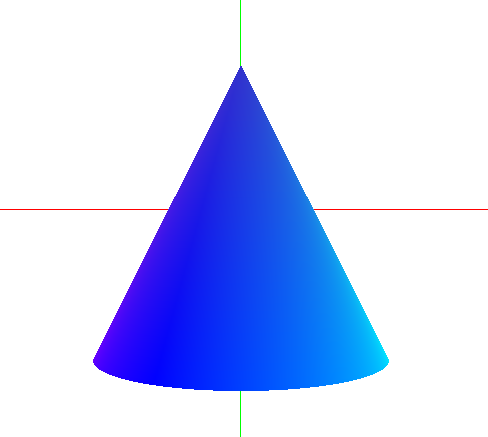
\includegraphics[width=\linewidth]{Imagenes/E6/act6_f1.png}
        \vspace{1mm}
        {\footnotesize (a) Vista frontal (F1).}
    \end{minipage}\hfill
    \begin{minipage}{0.31\textwidth}
        \centering
        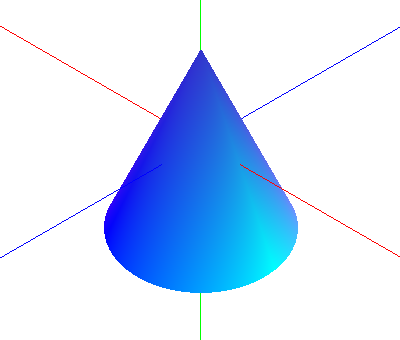
\includegraphics[width=\linewidth]{Imagenes/E6/act6_f2.png}
        \vspace{1mm}
        {\footnotesize (b) Vista oblicua (F2).}
    \end{minipage}\hfill
    \begin{minipage}{0.31\textwidth}
        \centering
        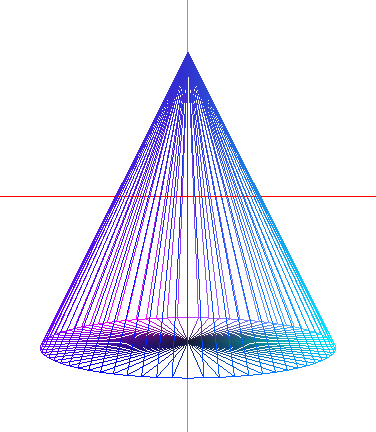
\includegraphics[width=\linewidth]{Imagenes/E6/act6_alambre.png}
        \vspace{1mm}
        {\footnotesize (c) Modo alambre (L).}
    \end{minipage}
    \vspace{2mm}
    \caption{Pruebas de visualización del cono de radio 1 y altura 2 centrado en el origen.}
    \label{fig:experimento_cono}
\end{figure}

\subsection{Actividad 7: Escena con OpenGL}

Para los experimentos se modificaron únicamente las transformaciones y los colores de algunos objetos de la escena, cambiando un solo objeto por cada tipo de transformación para poder compararlos contra el resultado original. Los cuatro cambios se aplicaron al mismo tiempo y se pueden ver en la Figura~\ref{fig:experimento_escena}.

En el primer experimento se cambió el escalamiento de la esfera roja de $(0.25,\,0.25,\,0.25)$ a $(0.25,\,0.25,\,0.5)$ y su centro se subió de $y=0.25$ a $y=0.5$ para que siguiera apoyada en el piso. La esfera se convirtió en un óvalo alargado de forma vertical, aunque el escalamiento se hizo en el eje $z$. Esto pasa porque el escalamiento se aplica antes que la rotación de $90^\circ$ respecto al eje $x$, y esa rotación convierte el eje $z$ local de la esfera en el eje vertical de la escena, lo que confirma que el orden $T\,R\,S$ de las transformaciones sí afecta el resultado.

En el segundo experimento se cambió la rotación del cono grande de $-90^\circ$ a $-60^\circ$ respecto al eje $x$. El techo dejó de estar derecho sobre la casa y quedó inclinado $30^\circ$, por lo que ahora se alcanza a ver parte de su base y ya no cubre de forma pareja al cilindro.

En el tercer experimento se trasladó el tercer árbol de $x=-2$ a $x=2$, moviendo tanto el tronco como las hojas con los mismos valores en $x$ y $z$. El árbol quedó del lado derecho de la escena, frente a la casa, sin separarse. Esto se debe a que el tronco y las hojas son objetos independientes con su propia matriz de modelo, así que para mover el árbol completo fue necesario aplicar la misma traslación a los dos.

Por último, en el cuarto experimento se cambiaron los colores de la casa: el cilindro pasó de naranja barro a azul grisáceo, con $(0.35,\,0.45,\,0.60)$, y el techo de beige a rojo teja, con $(0.70,\,0.15,\,0.10)$. El cambio se reflejó sin afectar al resto de los objetos, ya que cada uno tiene su propia malla con los colores asignados en sus vértices.

\begin{figure}[H]
    \centering
    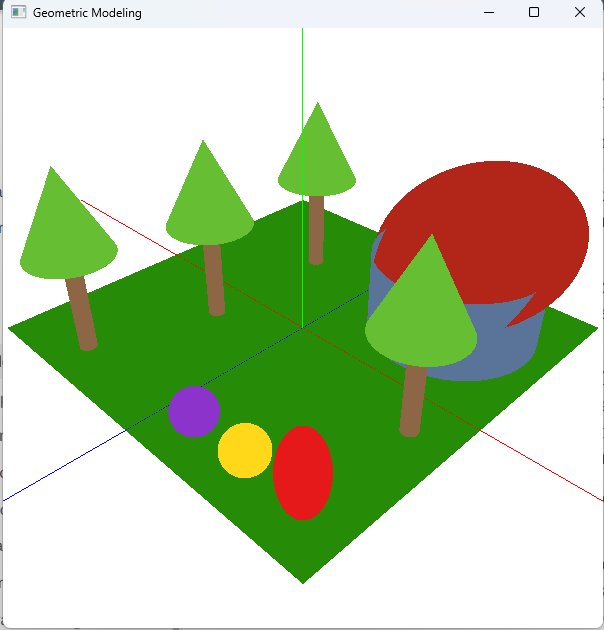
\includegraphics[width=0.6\textwidth]{Imagenes/E7/Escena_ex1.png}
    \caption{Escena con los cuatro experimentos aplicados: esfera roja escalada, techo rotado $-60^\circ$, tercer árbol trasladado a la derecha y nuevos colores de la casa, vista oblicua (F2).}
    \label{fig:experimento_escena}
\end{figure}